\documentclass[11pt]{article}

\usepackage[margin=1in]{geometry}
\usepackage{graphicx}
\usepackage{booktabs}
\usepackage{amsmath}
\usepackage{float}
\usepackage{listings}
\usepackage{xcolor}
\usepackage{subcaption}
\usepackage{longtable}

\lstset{
    basicstyle=\ttfamily\scriptsize,
    breaklines=true,
    breakatwhitespace=true,
    frame=single,
    columns=fullflexible
}

\title{Project 2: Regression and Symbolic Regression}
\author{Seth Cohen, Mahimna Patel, Krish Ranawat}
\date{\today}

\begin{document}
\maketitle

\section*{Overview}
This report extends the Project 1 exploratory analysis of three UCI datasets
(Auto MPG, Concrete Compressive Strength, Airfoil Self-Noise) with regression
and symbolic regression. Five techniques are evaluated using
\textbf{ScalaTion}, Python's \textbf{Statsmodels}, and \textbf{PySR}, following
the model allocation in the assignment:
\begin{enumerate}
    \item \textbf{Regression} (ScalaTion + Statsmodels): all 3 datasets.
    \item \textbf{Regularized Regression}, Ridge and Lasso (ScalaTion +
    Statsmodels): Auto MPG only.
    \item \textbf{Forward Feature Selection} (ScalaTion): Auto MPG and
    Concrete.
    \item \textbf{Transformed Regression}, log/sqrt/Box-Cox (ScalaTion): Auto
    MPG and Airfoil.
    \item \textbf{Symbolic Regression} (ScalaTion + PySR): all 3 datasets.
\end{enumerate}
Unless noted otherwise, models use every available predictor for a dataset
(no manual feature pre-selection), so results here are not directly comparable
to Project~1's two-feature simple regressions. Full console logs for every
ScalaTion run are in \texttt{results/<dataset>/scalation\_output.txt}; a
compact digest of coefficients and QoF is in
\texttt{results/<dataset>/scalation\_digest.txt}.

\clearpage
\section{Regression}

\subsection{Auto MPG}
ScalaTion's \texttt{Regression} and Statsmodels' \texttt{OLS} were fit on
\texttt{mpg} against all 7 predictors (\texttt{cylinders}, \texttt{displacement},
\texttt{horsepower}, \texttt{weight}, \texttt{acceleration},
\texttt{model\_year}, \texttt{origin}). Both tools solve the same
least-squares problem and, as expected, agree to at least 3 decimal places on
every coefficient and QoF metric.

\begin{table}[H]
\centering
\caption{Auto MPG multiple regression coefficients (ScalaTion; Statsmodels agrees).}
\begin{tabular}{lr}
\toprule
Term & Coefficient \\
\midrule
intercept & $-17.218$ \\
cylinders & $-0.4934$ \\
displacement & $0.01990$ \\
horsepower & $-0.01695$ \\
weight & $-0.006474$ \\
acceleration & $0.08058$ \\
model\_year & $0.7508$ \\
origin & $1.4261$ \\
\bottomrule
\end{tabular}
\end{table}

\textbf{QoF:} $R^2=0.8215$, adj.\ $R^2=0.8182$, RMSE $=3.294$, F(7,384)$=252.4$,
$p<0.001$. 5-fold cross-validation gives a very similar mean $R^2\approx0.81$
(fold range 0.62--0.84; see \texttt{scalation\_output.txt}), so the model
generalizes well and is not overfit.

\begin{figure}[H]
    \centering
    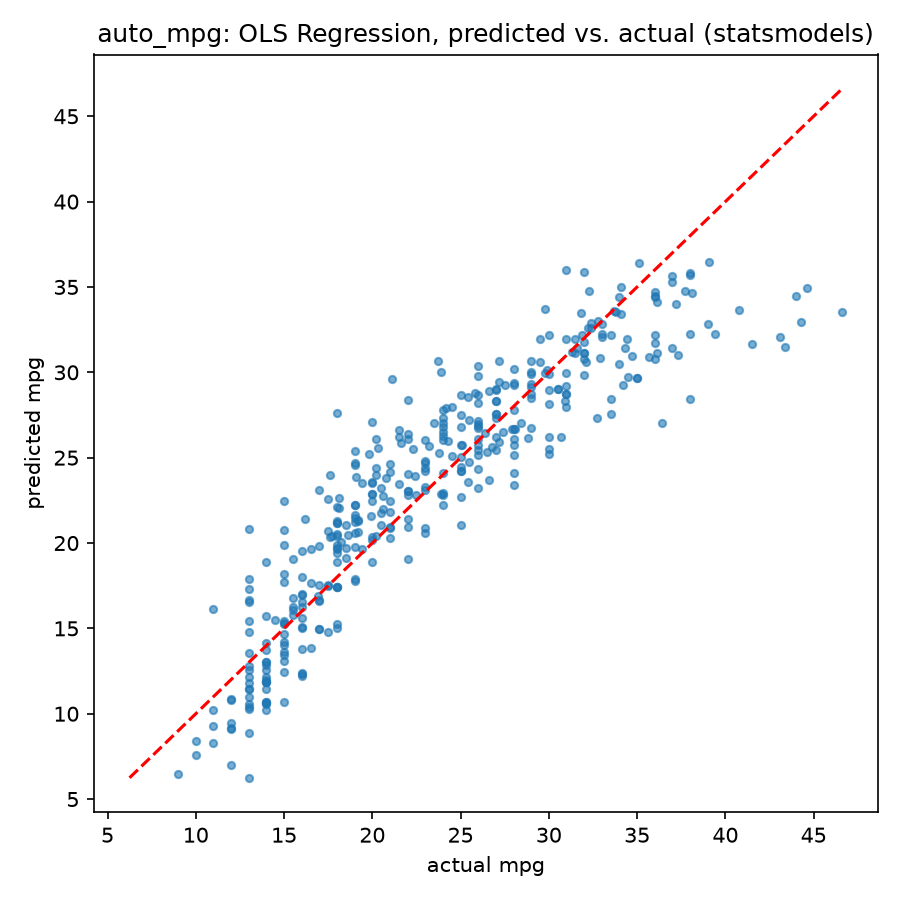
\includegraphics[width=0.55\textwidth]{../results/auto_mpg/fit_vs_actual_regression.png}
    \caption{Auto MPG: Statsmodels OLS, predicted vs.\ actual mpg.}
\end{figure}

\textbf{Interpretation:} weight, model\_year, and origin dominate: every
extra 1000 lbs costs about 6.5 mpg, each model year (1970--1982) is worth
about 0.75 mpg of efficiency gain, and non-US-built cars (origin 2/3) average
1.0--2.9 mpg higher after controlling for size and era. Cylinders is the only
predictor with a counter-intuitive sign once weight and displacement are held
constant, a sign of mild multicollinearity among the engine-size features
(cylinders, displacement, horsepower, weight are all highly correlated with
each other).

\subsection{Concrete Compressive Strength}
Regression of \texttt{concrete\_compressive\_strength} on all 8 ingredient
predictors.

\begin{table}[H]
\centering
\caption{Concrete multiple regression coefficients (ScalaTion; Statsmodels agrees).}
\begin{tabular}{lr}
\toprule
Term & Coefficient \\
\midrule
intercept & $-23.164$ \\
cement & $0.1198$ \\
blast\_furnace\_slag & $0.1038$ \\
fly\_ash & $0.0879$ \\
water & $-0.1503$ \\
superplasticizer & $0.2907$ \\
coarse\_aggregate & $0.0180$ \\
fine\_aggregate & $0.0202$ \\
age & $0.1142$ \\
\bottomrule
\end{tabular}
\end{table}

\textbf{QoF:} $R^2=0.6155$, adj.\ $R^2=0.6125$, RMSE $=10.35$.

\begin{figure}[H]
    \centering
    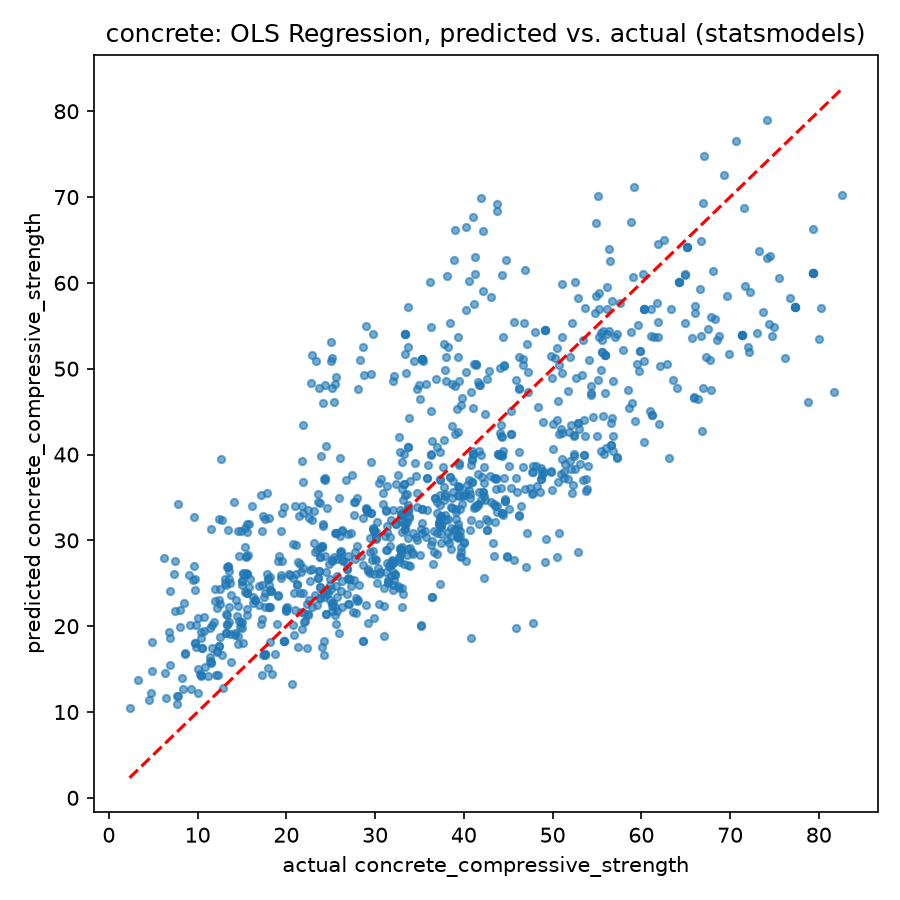
\includegraphics[width=0.55\textwidth]{../results/concrete/fit_vs_actual_regression.png}
    \caption{Concrete: Statsmodels OLS, predicted vs.\ actual compressive strength.}
\end{figure}

\textbf{Interpretation:} all three cementitious materials (cement, slag, fly
ash) and superplasticizer raise strength, while water lowers it, matching the
textbook water/cement-ratio relationship in concrete chemistry. Age has a
positive effect (curing), and the two aggregate fractions matter least. Using
all 8 predictors nearly doubles Project 1's best single-feature fit
($R^2\approx0.25$ for cement alone), confirming strength is genuinely
multivariate, but 38\% of the variance is still unexplained, likely due to
nonlinear curing/age interactions (addressed in Section 5).

\subsection{Airfoil Self-Noise}
Regression of \texttt{scaled\_sound\_pressure\_level} on all 5 predictors.

\begin{table}[H]
\centering
\caption{Airfoil multiple regression coefficients (ScalaTion; Statsmodels agrees).}
\begin{tabular}{lr}
\toprule
Term & Coefficient \\
\midrule
intercept & $132.83$ \\
frequency & $-0.001282$ \\
angle\_of\_attack & $-0.4219$ \\
chord\_length & $-35.69$ \\
free\_stream\_velocity & $0.09985$ \\
suction\_side\_displacement\_thickness & $-147.30$ \\
\bottomrule
\end{tabular}
\end{table}

\textbf{QoF:} $R^2=0.5157$, adj.\ $R^2=0.5141$, RMSE $=4.799$.

\begin{figure}[H]
    \centering
    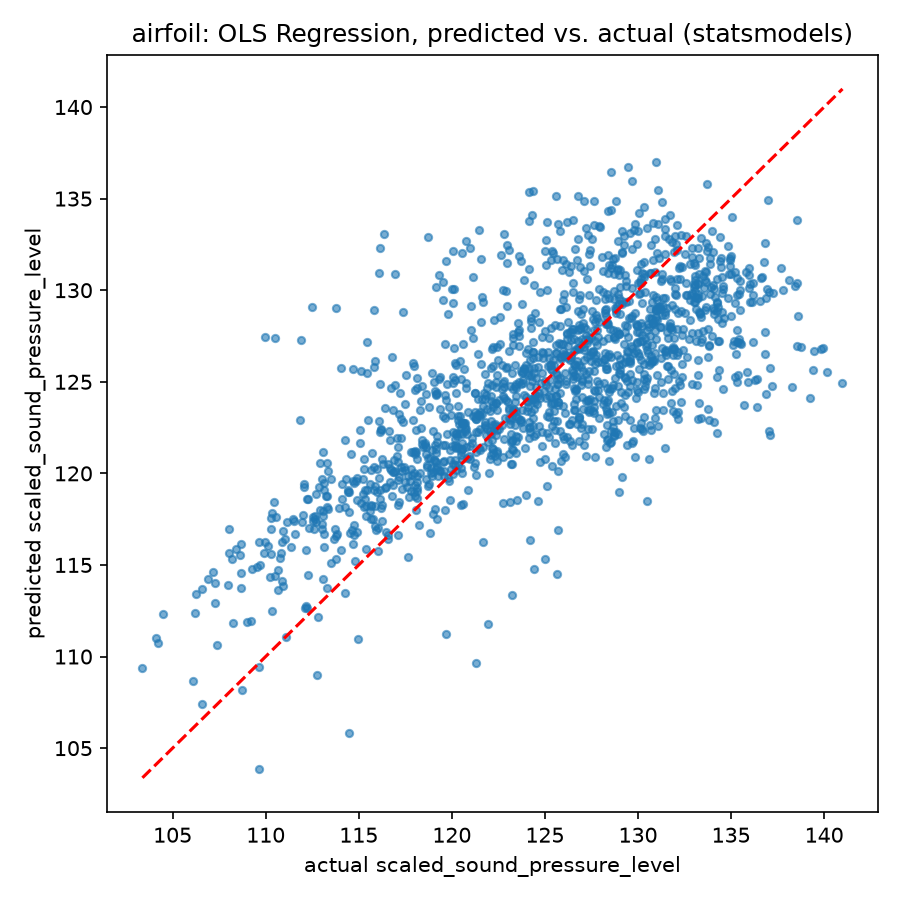
\includegraphics[width=0.55\textwidth]{../results/airfoil/fit_vs_actual_regression.png}
    \caption{Airfoil: Statsmodels OLS, predicted vs.\ actual sound pressure level.}
\end{figure}

\textbf{Interpretation:} higher free-stream velocity is the only predictor
that \emph{raises} noise, matching aerodynamics (faster flow means louder
self-noise); the other four all lower the fitted sound pressure level. Using
all 5 predictors more than triples Project 1's best single-feature fit
($R^2\approx0.15$ for frequency alone), but this remains the weakest linear
fit of the three datasets, consistent with the Project 1 finding that
boundary-layer self-noise is a genuinely nonlinear phenomenon.

\clearpage
\section{Regularized Regression (Auto MPG only)}
\begin{sloppypar}
Ridge (L2) and Lasso (L1) were fit on Auto MPG in both tools. ScalaTion's
\texttt{RidgeRegression}/\texttt{LassoRegression} auto-center $x$ and $y$
(coefficients are on the original predictor scale, no intercept term);
Statsmodels' \texttt{OLS.fit\_regularized} was run on standardized predictors.
For each of the four models, the penalty ($\lambda$ for ScalaTion, $\alpha$
for Statsmodels) was chosen by 5-fold cross-validated SSE/MSE over a grid
(see \texttt{results/auto\_mpg/\{ridge,lasso\}\_alpha\_search.csv} and the
\texttt{scalation\_output.txt} lambda-search log).
\end{sloppypar}

\begin{table}[H]
\centering
\caption{Auto MPG Ridge and Lasso: chosen penalty and in-sample fit.}
\begin{tabular}{llrr}
\toprule
Tool & Model & Penalty (CV-chosen) & $R^2$ \\
\midrule
ScalaTion & Ridge & $\lambda=10.0$ & 0.8214 \\
ScalaTion & Lasso & $\lambda=5.0$ & 0.8215 \\
Statsmodels & Ridge & $\alpha=0.05$ & 0.8154 \\
Statsmodels & Lasso & $\alpha=0.1$ & 0.8178 \\
\midrule
 & (unregularized OLS, Section 1) & -- & 0.8215 \\
\bottomrule
\end{tabular}
\end{table}

\begin{table}[H]
\centering
\caption{Statsmodels standardized coefficients: Ridge vs.\ Lasso (Auto MPG).}
\begin{tabular}{lrr}
\toprule
Predictor & Ridge & Lasso \\
\midrule
cylinders & $-0.609$ & $0.000$ \\
displacement & $0.152$ & $0.000$ \\
horsepower & $-0.989$ & $-0.381$ \\
weight & $-3.684$ & $-4.718$ \\
acceleration & $-0.096$ & $0.000$ \\
model\_year & $2.530$ & $2.646$ \\
origin & $1.056$ & $0.892$ \\
\bottomrule
\end{tabular}
\end{table}

\textbf{Interpretation:} with only 7 predictors on 392 rows, unregularized
OLS is not overfitting, so shrinkage barely moves $R^2$ (0.815--0.822 across
all four models, within noise of the CV grid search). The value of
regularization here is in \emph{variable importance}, not accuracy: Lasso's
L1 penalty drives \texttt{cylinders}, \texttt{displacement}, and
\texttt{acceleration} exactly to zero, leaving a sparse 3-predictor model
(\texttt{horsepower}, \texttt{weight}, \texttt{model\_year}, \texttt{origin})
that confirms the same story as the forward-selection order in Section 3:
weight and model year are the dominant drivers of fuel economy, and the
engine-size predictors are redundant with each other once weight is in the
model. ScalaTion's Ridge/Lasso (which do not standardize predictors) picked
much larger $\lambda$ before the CV-SSE curve turned upward, but told the same
qualitative story: \texttt{acceleration}'s coefficient shrinks the most under
Lasso ($0.0806\rightarrow0.0309$), while \texttt{weight} and
\texttt{model\_year} are essentially unchanged.

\clearpage
\section{Forward Feature Selection}
ScalaTion's \texttt{forwardSelAll} was run on Auto MPG and Concrete (Airfoil
was left out, since it has only 5 predictors -- too few for the ordering to
be very informative -- while the other two datasets have 7--8). By default
ScalaTion selects using sMAPE$_C$ (lower is better), not $R^2_{bar}$.

\subsection{Auto MPG}
\begin{quote}
\small\texttt{one $\rightarrow$ weight $\rightarrow$ model\_year $\rightarrow$
origin $\rightarrow$ cylinders $\rightarrow$ acceleration $\rightarrow$
displacement $\rightarrow$ horsepower}
\end{quote}
The cross-validated sMAPE$_C$ improves at every step (11.9 $\rightarrow$ 6.98)
and is minimized only once all 7 predictors are included ($R^2_{bar}=0.818$,
matching Section 1's full model). No smaller subset outperforms the full
model.

\subsection{Concrete}
\begin{quote}
\small\texttt{one $\rightarrow$ superplasticizer $\rightarrow$ age $\rightarrow$
cement $\rightarrow$ blast\_furnace\_slag $\rightarrow$ fly\_ash
$\rightarrow$ water $\rightarrow$ fine\_aggregate $\rightarrow$
coarse\_aggregate}
\end{quote}
Same pattern: sMAPE$_C$ falls monotonically (38.6 $\rightarrow$ 26.7) and the
full 8-predictor model is best ($R^2_{bar}=0.612$).

\textbf{Interpretation:} in both datasets every predictor pulls its weight
statistically, so forward selection does not reduce dimensionality --- its
value here is the \emph{order} in which features are added, which is a
model-based importance ranking. For Auto MPG that ranking (weight, then
model\_year, then origin) matches the Lasso sparsity pattern in Section 2
almost exactly. For Concrete, superplasticizer and age are selected before
cement, showing that once workability (superplasticizer) and curing time
(age) are accounted for, raw cement content adds comparatively less marginal
predictive power than its Section 1 coefficient alone would suggest.

\clearpage
\section{Transformed Regression}
ScalaTion's \texttt{TranRegression} was run on Auto MPG and Airfoil,
applying \texttt{log(y)}, \texttt{sqrt(y)}, and Box-Cox($y$)
with $\lambda=0.4$ (the library default; Yeo-Johnson is not exposed as a
ready-made \texttt{Transform} in this ScalaTion build, so Box-Cox was used, as
permitted by the rubric). Both target variables are strictly positive, so all
three transforms are well-defined.

\begin{table}[H]
\centering
\caption{Effect of transforming the response on in-sample $R^2$.}
\begin{tabular}{lrrrr}
\toprule
Dataset & Untransformed & log($y$) & sqrt($y$) & Box-Cox($y$), $\lambda=0.4$ \\
\midrule
Auto MPG (mpg) & 0.8215 & \textbf{0.8552} & 0.8437 & 0.8468 \\
Airfoil (dB) & \textbf{0.5157} & 0.5082 & 0.5122 & 0.5114 \\
\bottomrule
\end{tabular}
\end{table}

\textbf{Interpretation:} the two datasets tell opposite stories, which is
itself the interesting finding. \texttt{mpg} is a reciprocal-like, right-skewed
quantity (efficiency measured as distance/fuel rather than the more
physically additive fuel/distance), so every transform toward a
more-symmetric scale improves the fit; log is best, gaining $\Delta R^2
\approx 0.034$ over the untransformed model, consistent with standard
practice of regressing $\log(\text{mpg})$ or gallons-per-100-miles instead of
mpg directly. \texttt{scaled\_sound\_pressure\_level}, by contrast, is
\emph{already} a decibel (logarithmic) quantity, so applying a further
log/sqrt/Box-Cox transform does not help and mildly hurts every metric,
because it fights against a scale that is already close to linear in the
underlying physics. This is a clean illustration that transformed regression
should be guided by the target's native scale, not applied by default.

\clearpage
\section{Symbolic Regression}
Both a power/cross-term expansion in ScalaTion and a genetic symbolic search
in PySR were run on all three datasets.

\subsection{ScalaTion}
Each dataset's predictors were expanded with $x^{0.5}$, $x^{2}$, an
intercept, and all pairwise cross terms $x_ix_j$, then \texttt{forwardSelAll}
was used to rank terms (as in Section 3, this ranks by cross-validated
sMAPE$_C$, lower is better). An earlier attempt that also included $x^{-1}$
and $x^{-0.5}$ terms produced a severely multicollinear, numerically unstable
design matrix (coefficients up to $10^{15}$, NaN standard errors, and an
outright crash on Concrete) since a variable's reciprocal and direct powers
are highly correlated; the power set was narrowed to $\{0.5,2\}$ to keep the
expansion well-conditioned.

\begin{table}[H]
\centering
\caption{ScalaTion symbolic regression: full expanded model vs.\ best
cross-validated subset from forward selection.}
\begin{tabular}{lrrrrr}
\toprule
Dataset & Terms (full) & $R^2$ (full) & Best subset size & sMAPE$_C$ (best) & sMAPE$_C$ (full) \\
\midrule
Auto MPG & 36 & 0.8946 & 27 of 36 & 6.979 & 7.063 \\
Concrete & 45 & 0.8857 & 37 of 45 & 13.27 & 14.23 \\
Airfoil & 21 & 0.6411 & 16 of 21 & 2.503 & 2.517 \\
\bottomrule
\end{tabular}
\end{table}

\textbf{Interpretation:} for Auto MPG the sMAPE$_C$ curve is nearly flat from
about 19--31 terms (6.98--7.00), so forward selection finds no compact,
clearly-superior subset -- symbolic expansion buys a real accuracy gain over
linear regression ($R^2$: 0.89 vs.\ 0.82) but needs most of the expanded
basis to get it. Concrete is the more instructive case: cross-validated
sMAPE$_C$ improves steadily through 37 terms and then \emph{worsens} for the
last 8 (superplasticizer\_cement, fine\_aggregate$^2$, age\_coarse\_aggregate,
age\_cement), a textbook sign that those late-added terms are fitting noise
rather than signal; the 37-term subset generalizes better than the full
45-term model despite the full model's higher in-sample $R^2$. Airfoil's
best subset (16 of 21 terms, $R^2=0.64$) is a real improvement over Section 1
($R^2=0.52$) but is still the weakest of the three datasets, again pointing
to nonlinear structure beyond what a low-order power/cross-term basis
captures.

\subsection{PySR}
PySR (binary operators $+,-,\times,\div$; unary operators
$\mathrm{square}, \mathrm{sqrt}, \exp, \log$; 60 iterations, population size
33) searched directly over closed-form expressions rather than a fixed basis.

\begin{table}[H]
\centering
\caption{PySR best equation per dataset (selected by PySR's complexity/loss
score).}
\begin{tabular}{p{0.13\textwidth}p{0.62\textwidth}rr}
\toprule
Dataset & Equation & Complexity & $R^2$ \\
\midrule
Auto MPG & $\text{mpg} = \dfrac{(\text{model\_year} - 45.714)\times 2104.74}{\text{weight}}$ & 7 & 0.8508 \\[8pt]
Concrete & $\text{strength} = \dfrac{\log(\text{fly\_ash}+\text{water})\,(\log(\text{age})\,\text{cement}+958.16)}{\text{water}} + \sqrt{\text{blast\_furnace\_slag}} - 24.85$ & 18 & 0.7564 \\[10pt]
Airfoil & $\text{spl} = 131.38 - \sqrt{25.816\;\text{freq}\cdot\text{chord}\cdot\text{thickness}}$ & 10 & 0.5556 \\
\bottomrule
\end{tabular}
\end{table}

\begin{figure}[H]
    \centering
    \begin{subfigure}{0.32\textwidth}
        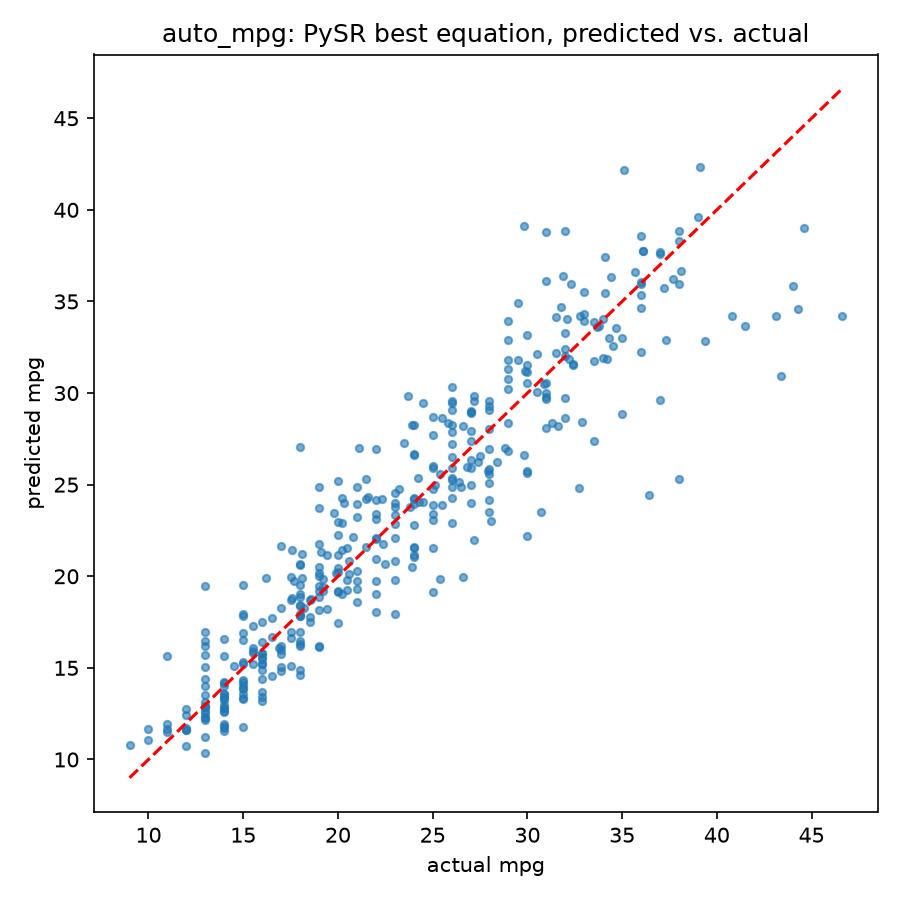
\includegraphics[width=\textwidth]{../results/auto_mpg/pysr_fit_vs_actual.png}
        \caption{Auto MPG}
    \end{subfigure}
    \begin{subfigure}{0.32\textwidth}
        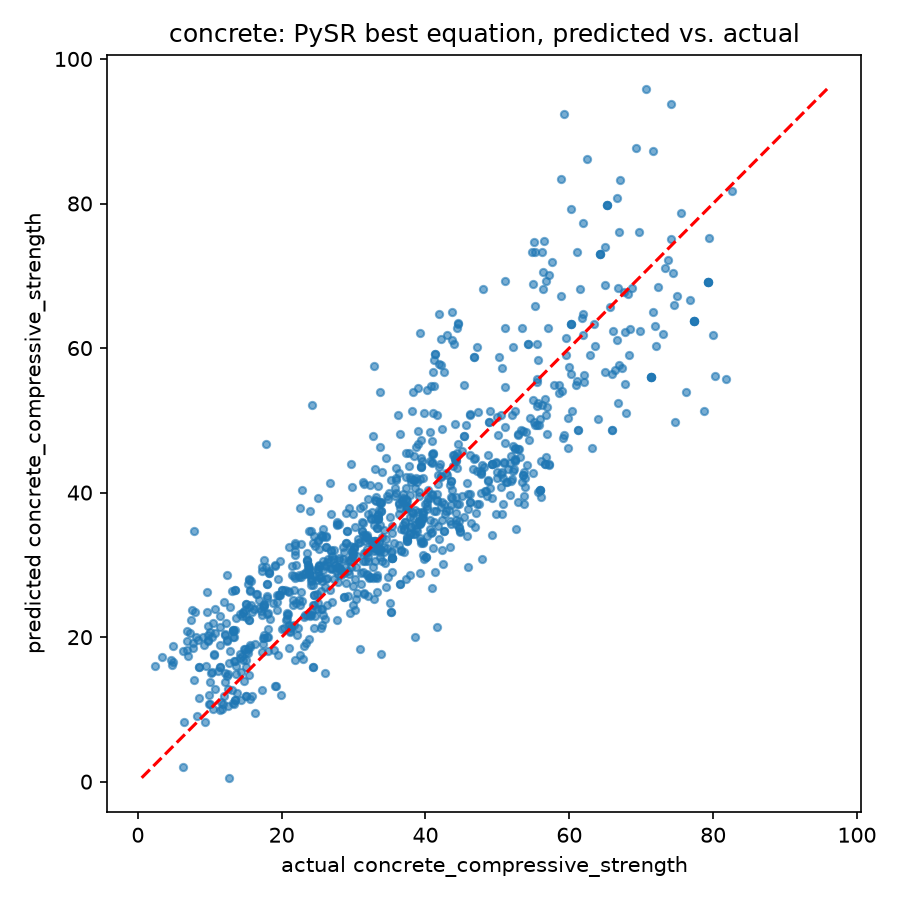
\includegraphics[width=\textwidth]{../results/concrete/pysr_fit_vs_actual.png}
        \caption{Concrete}
    \end{subfigure}
    \begin{subfigure}{0.32\textwidth}
        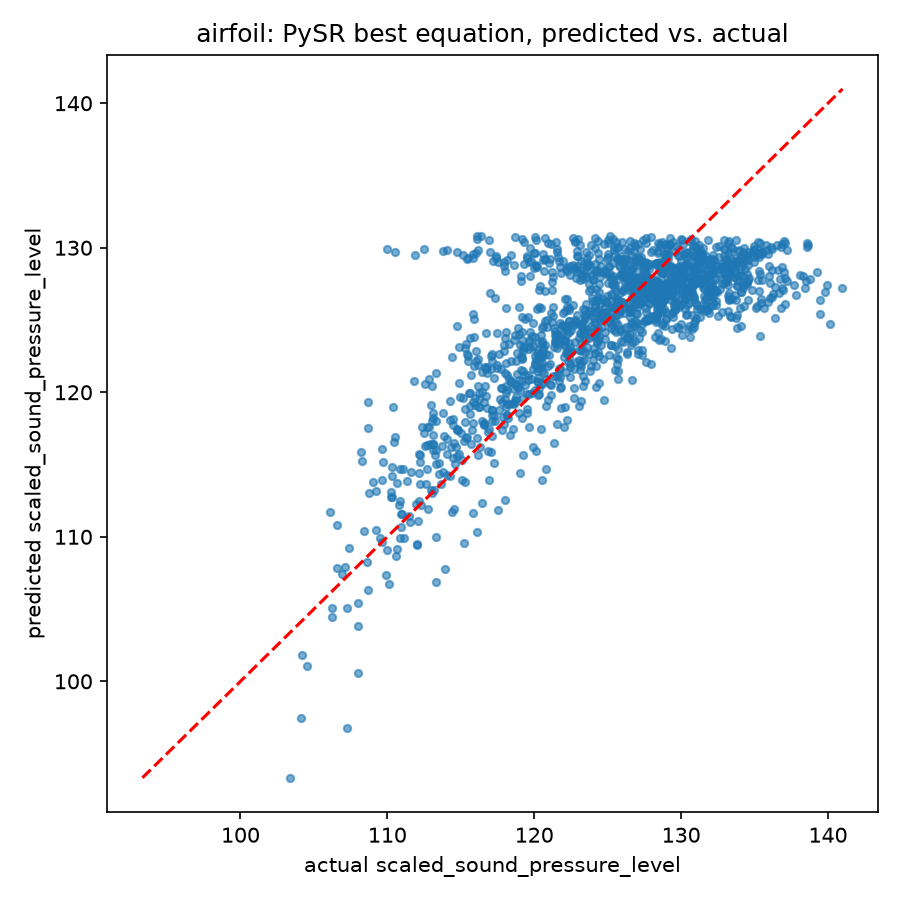
\includegraphics[width=\textwidth]{../results/airfoil/pysr_fit_vs_actual.png}
        \caption{Airfoil}
    \end{subfigure}
    \caption{PySR best-equation predictions vs.\ actual, all three datasets.}
\end{figure}

\textbf{Interpretation:} PySR's Auto MPG equation is remarkably close to
physical reasoning -- it rediscovers, essentially unprompted, that fuel
economy scales with a (model-year-adjusted) constant divided by weight, using
only 2 fitted constants for $R^2=0.851$, nearly matching the 8-parameter
linear model ($R^2=0.822$) with far fewer degrees of freedom. For Concrete,
PySR clearly outperforms both the linear model ($R^2=0.616$) and is
competitive with ScalaTion's much larger power-basis expansion, by finding a
$\log(\text{age})\times\text{cement}/\text{water}$ interaction term that a
low-order polynomial basis cannot represent directly -- this lines up with
concrete science, where strength gain follows a roughly logarithmic curing
curve in age and depends multiplicatively on the cement/water ratio. For
Airfoil, PySR's compact equation ($R^2=0.556$) improves modestly on linear
regression and is close to, though below, ScalaTion's larger 16-term
expansion ($R^2=0.641$); the shared \texttt{frequency}
$\times$~\texttt{chord\_length}~$\times$~\texttt{thickness} product it finds
matches known airfoil self-noise scaling laws (noise grows with these
geometric/aerodynamic products), but the modest $R^2$ across every method in
this section confirms that a large share of Airfoil's noise variance is not
captured by low-order combinations of these five predictors.

\clearpage
\section*{Cross-Section Summary}
\begin{itemize}
    \item \textbf{Regression accuracy ranks consistently as Auto MPG $>$
    Concrete $>$ Airfoil} across every section (Regression, Symbolic
    Regression), reflecting how linear/near-linear each underlying physical
    process is.
    \item \textbf{Regularization} (Section 2) matters for interpretability
    (Lasso's sparsity confirms which of Auto MPG's correlated engine-size
    features are redundant) more than for raw accuracy, since the
    unregularized model was not overfitting to begin with.
    \item \textbf{Forward selection} (Section 3) did not shrink either model
    -- both datasets' predictors are each informative -- but its ordering
    corroborates the Lasso sparsity pattern.
    \item \textbf{Transformed regression} (Section 4) only helps when the
    transform matches the target's native scale: it clearly helped Auto MPG
    (already skewed) and did not help Airfoil (already log-scaled in dB).
    \item \textbf{Symbolic regression} (Section 5) gave the largest accuracy
    gains of any technique for Concrete and Auto MPG, and in both PySR's
    genetic search and ScalaTion's power-basis expansion recovered terms
    (a $1/\text{weight}$ scaling; a $\log(\text{age})$ curing term) that
    have clear physical/engineering justification, not just statistical
    ones.
\end{itemize}

\end{document}
